
\documentclass[13pt]{jarticle}


\title{2019年に得たフローの知見について}
\author{tokoharu}

\date {2019.12.25 }

\usepackage{amsthm}
\usepackage{algorithm}
\usepackage{algorithmic}
\usepackage{ascmac}
\usepackage{amsmath}
\usepackage{courier}
%\usepackage{eqnarray}
\usepackage[dvipdfmx]{graphicx}
\usepackage{helvet}
\usepackage{times}
\setlength{\textwidth}{17cm}
\setlength{\textheight}{23cm}
\setlength{\oddsidemargin}{-0.5cm}
\setlength{\evensidemargin}{-0.5cm}
\setlength{\topmargin}{-1cm}
%\usepackage{ascmac}
%\usepackage{here}
\usepackage{txfonts}
\usepackage{listings}
\usepackage{lscape}
\usepackage{url}
\usepackage[dvipdfmx]{hyperref}
\usepackage{pxjahyper}
\usepackage{wrapfig}


% tikz
\usepackage{tikz}
\usetikzlibrary{calc}
\usetikzlibrary{arrows}
\usetikzlibrary{math}

\tikzset{%
  myedge/.style={->, shorten >=1pt, >=triangle 60},
  mynode/.style={circle, draw=black }
}

% sourcecode
\lstset{
  basicstyle={\ttfamily},
  identifierstyle={\small},
  commentstyle={\smallitshape},
  keywordstyle={\small\bfseries},
  ndkeywordstyle={\small},
  stringstyle={\small\ttfamily},
  frame={tb},
  breaklines=true,
  columns=[l]{fullflexible},
  numbers=left,
  xrightmargin=0zw,
  xleftmargin=3zw,
  numberstyle={\scriptsize},
  stepnumber=1,
  numbersep=1zw,
  lineskip=-0.5ex
}



\begin{document}
\maketitle




\section{全体のイントロ}
この記事は次のとおり,二部構成となっています.

前半は「普通に考えると最小費用流なのに$O(N)$や$O(N \log N)$程度の計算量を要求されてしまう...」という類の問題についてです.この問題へのアプローチと例題の解説をします.
紹介する問題 : JOI2018/2019 本選 問題4「コイン集め」

後半は「グリッド上の最大流」になります.左上から右下へ容量無限大の辺を無数に張られていて,ソースとシンクがたくさんあるような設定の最大流について扱います.
紹介する問題 : いろはちゃんコンテストDay4 F「道なき道を」, JOI2018/2019 春合宿 Day2 「ふたつの料理」

想定読者層は,最大流問題,最小費用流問題について,それぞれ問題を解いたことがあるのが最低ラインだと思います.(特に何の理由もつけずに,「この問題はナイーブなフローで解けますね~」,くらいの説明をすることになります)



\section{ (前半)高速化できる最小費用流のよくあるからくり}

\begin{figure}[htbp]
\centering
\begin{tabular}{c}
\begin{minipage}{0.3\hsize}
\centering
\begin{tikzpicture}

  \tikzset{myedge/.style={->, shorten >=1pt, >=triangle 60}};
  \tikzset{mynode/.style={circle, draw=black }};
  \node[mynode] (s) {$s$};
  \node[mynode,right=3cm] (t) at (s) {$t$};
  \node[mynode,right=1.5cm, above=0.5cm] (a) at (s) {};
  \node[mynode,right=1.5cm, below=0.5cm] (b) at (s) {};
  \node [left=1cm](X) at (s) {};


  \draw [myedge] (s.east) -- (a.west) ;
  \draw [myedge] (s.east) -- (b.west);
  \draw [myedge] (a.east) -- (t.west);
  \draw [myedge] (b.east) -- (t.west);
  \draw [myedge] (a.south) -- (b.north);
  \draw [myedge] (X) -- (s.west) node [midway, above] {$x$};
\end{tikzpicture}
\end{minipage}

\begin{minipage}{0.1\textwidth}
\centering
\begin{tikzpicture}
\node {$\Leftrightarrow$};
\end{tikzpicture}
\end{minipage}

\begin{minipage}{0.4\hsize}
\centering

\begin{tikzpicture}
\coordinate (O) at (0,0);
\coordinate (AX) at (-1,0); \coordinate(BX) at (6,0);
\coordinate (AY) at (0,-0.5); \coordinate(BY) at (0,5);
\draw[->, >=triangle 60] (AX) -- (BX); \draw[->, >=triangle 60] (AY) -- (BY);
\node at (BX) [below=0.1] {$x$};
\node at (BY) [right=0.1] {$f(x)$};

\coordinate (P) at (3, 1); \coordinate (Q) at (1, 0); \coordinate (R) at (5, 5);
\coordinate (Z) at (-0.5, 4);
\node(S) at (3,0)[below=0.1] {3};
\node [below=0.1] at (Q) {$1$};
\node (T) at (0,1) [left=0.1] {1};
\draw (Z) -- (Q) -- (P) -- (R);
\draw [dotted] (P) -- (S);
\draw [dotted] (P) -- (T);



\end{tikzpicture}

\end{minipage}
\end{tabular}

\caption{対応のイメージ(最小費用流と区分線形関数)}

\end{figure}



\subsection{イントロ}

最小費用流問題に帰着できる問題の中でも,「なぜかよくわからんけれど性質がいいからいつの間にか高速化できてしまうような問題」が出題されることがたまにあります.
この記事ではそのからくりにおける考え方をご紹介したいと思います.

まず,この話のベースになっているのはwataさんがtwitterで紹介されていた論文になります.
この論文について,細かい実装は省略し,その考え方をざっくり説明します.
そのあとで,実際の問題への適用例を紹介していきます.

なお,今回紹介する考え方で面白いことなのですが,この論文にある考え方を用いることで,アドホックに見えるアルゴリズム自体を構成できるということです.
つまり,論文中で説明されているアルゴリズムが書かれたプログラムをライブラリとして用意している必要はないということです(こんなことを書くと,本当に必要になってしまう問題が作られてしまいそうですが).
なぜこのようなことが起きるのかというと,部分問題だったとしても素で出題されると十分に難しい問題だと思われるうえに,解法を読んでもあまりパターン化できる印象を受けず,アドホックなアルゴリズムだと捉えられるからだと考えています.


\subsection{論文で書かれていること}
対象となる論文は次です(\url{https://www.sciencedirect.com/science/article/pii/S0196677496900450})

この論文で言いたいことは,$G$上の$s - t$最小費用流のインスタンスについて,$(G, s, t)$が次の手順で構成可能な時,このインスタンスは高速に解くこと出来るということです.

\begin{itemize}
\item $G$は頂点$s, t$のみを持ち,その間に辺が張られており、その辺のコストは流量に対して区分線形凸関数になっている\footnote{競プロの文脈で登場する設定ではコストの条件は満たしていると言っていいでしょう.流量制約が無ければ単に一次関数ですし,最小流量・最大流量がある場合には,制約の外のコストを$\infty$にすればよいからです.また,区分線形関数は流量が負でも扱えるため,辺の向きも特に気にする必要がありません.}
\item 構成できた2つのインスタンス$(G_1, s_1, t_1)$と$(G_2, s_2, t_2)$に対して,$t_1=s_2$として頂点を一体化したグラフ$(G, s_1, t_2)$(以後,直列つなぎと呼びます)
\item 構成できた2つのインスタンス$(G_1, s_1, t_1)$と$(G_2, s_2, t_2)$に対して,$s_1=s_2, t_1=t_2$としたグラフ$(G, s_1, t_1)$(以後,並列つなぎと呼びます)
\end{itemize}

なお,このような手順で構成できるグラフから成るグラフクラスはSeries-parallel graphと呼ばれています. 
上記構成手順はリンク先の図を見るとよりイメージしやすいかもしれません.
\url{https://en.wikipedia.org/wiki/Series-parallel_graph}


\begin{figure}

\centering

\begin{tabular}{c}
\begin{minipage}{0.45\textwidth}
\centering
\begin{tikzpicture}
  \node[mynode] (z) {$s$};
  \node[mynode,left=2cm, below=2cm] (x1) at (z) {$t$};
  \node[mynode,right=2cm] (x2) at (x1) {$a$};
  \node[mynode,right=4cm] (x3) at (x1) {$b$};

  \draw (z.west) -- (x1.north) ;
  \draw (z.south) -- (x2.north);
  \draw (z.east) -- (x3.north);
  \draw (x1.east) -- (x2.west);
  \draw (x2.east) -- (x3.west);
  
\end{tikzpicture}
\end{minipage}
  
\hfill
\begin{minipage}{0.45\textwidth}
\centering
\begin{tikzpicture}
  \coordinate (x0) ;
  \coordinate[left=2cm, below=1cm] (x1) at (x0) ;
  \coordinate[right=4cm] (x2) at (x1) ;
  \coordinate[left=1cm, below=3cm] (x3) at (x0) ;
  \coordinate[right=2cm] (x4) at (x3) ;
  
  \draw (x0) -- (x1) -- (x2) -- (x3) -- (x4) -- (x0);
  \draw (x0) -- (x2) -- (x4) -- (x1) -- (x3) -- (x0);
  
\end{tikzpicture}
\end{minipage}
\end{tabular}
\caption{構成できるグラフの例 / 構成できないグラフの例}
\label{fig_ex1}	
\end{figure}

構成できる例とできない例をそれぞれ図$\ref{fig_ex1}$に示します.
前者は辺$sb$,辺$ba$を作成し,これを直列につなぎ,辺$sa$と並列につなぎ,さらに辺$at$と直列につなぎ,最後に辺$st$と並列につなぐことで構成することができます.
後者については不可能です.構成法よりSeries-parallel graphの平面性が言える一方で,このグラフは平面性がないからです.


では,上記インスタンスはどうして高速に解けるのか,そのトリックを簡単に説明します.
まず,一般に最小費用流問題において,流量$x$を動かしたときの最小費用流の答えがどうなるか,関数だと思って描けばその関数形は区分線形凸関数になります.
ポイントは,上記にあげた2つの操作(直列/並列つなぎ)はこの区分線形凸関数に対する演算だと考えることができるという点です.

具体的には,次のようになります.
\begin{itemize}
\item 直列につなぐ : 単純な足し算 $f(x) = g(x) + h(x)$
\item 並列につなぐ : 畳み込み演算 $f(x) = \min_y {g(y) + h(x-y)}$
\end{itemize}
結局これらの演算を高速に行うことができるため,全体の最小費用流の解も高速に求めることができる,というのがトリックでした.

ここで,単純な足し算はともかく,畳み込み演算については第一印象で扱いづらそうに見える演算です.
しかしながら,区分線形凸関数における畳み込み演算は意外と簡単に計算できます.
このことがわかる定理を紹介します.

\begin{itembox}[l]{畳み込み演算の性質}
$g(x) \geq 0, h(x) \geq 0, g(0)=0, h(0)=0$を満たす,区分線形凸関数$g,h$を用意します.
畳み込みの結果である$f(x)$は,$f(0)=0$で,そこから$x$座標の増加方向への形状は,
$g(x)$, $h(x)$の$x\geq 0$に現れる線分について,傾きの順にソートして,
順に並べることで構成できる.

(\url{https://hal.archives-ouvertes.fr/hal-00281355/document} theorem 5, Figure3など)
\end{itembox}
上記定理では簡単のため,$x=0$を最小となる点としていますが,一般の区分線形凸関数について同様のことが成り立ちます.
また,説明では$x \geq 0$としているため,最小点から右側の領域しか見ていませんが,
左側の領域についても同様の性質を持ちます.


具体的な計算を例を挙げて説明しましょう.
$g(x) = 
\begin{cases}
0 & (0 \leq x \leq 1) \\
 \infty &  (\text{otherwise})
\end{cases}
, h(x) = abs(x)$とします.

\begin{figure}[htbp]
\begin{tabular}{r}

\begin{minipage}{0.45\textwidth}
\centering

\begin{tikzpicture}
\coordinate (O) at (2,0);
\coordinate (AX) at (1,0); \coordinate(BX) at (7,0);
\coordinate (AY) at (3,-0.5); \coordinate(BY) at (3,5);
\draw[->, >=triangle 60] (AX) -- (BX); \draw[->, >=triangle 60] (AY) -- (BY);

\coordinate (P) at (3, 4) ;
\coordinate (Q) at (4,4) ;
\coordinate (Pleft)  at (1, 4) ;
\coordinate (Qright) at (6, 4) ;
\coordinate (R) at (3, 0);
\coordinate (S) at (4, 0);

\node [right] at (P) {$\infty$}; 
\node [below] at(S) {1};

\draw [red, dotted, ultra thick] (P) -- (R);
\draw [red, dotted, ultra thick] (Q) -- (S);
\draw [red, ultra thick] (P) -- (Pleft);
\draw [red, ultra thick] (Q) -- (Qright);
\draw [red, ultra thick] (R) -- (S);

\node at (BX) [below=0.2] {$x$};
\node at (BY) [right=0.1] {$g(x)$};

\coordinate (P) at (3,0); \coordinate (Q) at (-0.5,3.5); \coordinate (R) at (6.5, 3.5);
\node (T) at (0,0){};
\node [below right] at (P){0};


\end{tikzpicture}
\end{minipage}


\begin{minipage}{0.45\textwidth}
\centering

\begin{tikzpicture}
\coordinate (O) at (2,0);
\coordinate (AX) at (0, 0); \coordinate(BX) at (6,0);
\coordinate (AY) at (3,-0.5); \coordinate(BY) at (3,5);
\draw[->, >=triangle 60] (AX) -- (BX); \draw[->, >=triangle 60] (AY) -- (BY);
\node at (BX) [below=0.2] {$x$};
\node at (BY) [right=0.1] {$h(x)$};

\coordinate (P) at (3,0); \coordinate (Q) at (0.5,2.5); \coordinate (R) at (5.5, 2.5);
\node (T) at (0,0){};
\node (ZERO) at (3.2, -0.2){0};
\draw (Q) -- (P) node [midway, right=0.2] {傾き $-1$};
\draw (P) -- (R) node [midway, right=0.2] {傾き $1$};
\draw [dotted] (P) -- (S);
\draw [dotted] (P) -- (T);


\end{tikzpicture}
\end{minipage}
\end{tabular}
\caption{畳み込み演算をする前}
\label{convolution_1}
\end{figure}


\begin{figure}[htbp]
\centering
\begin{tikzpicture}


\coordinate (O) at (2,0);
\coordinate (AX) at (-1, 0); \coordinate(BX) at (7,0);
\coordinate (AY) at (2,-0.5); \coordinate(BY) at (2,5);
\draw[->, >=triangle 60] (AX) -- (BX); \draw[->, >=triangle 60] (AY) -- (BY);
\node at (BX) [below=0.2] {$x$};
\node at (BY) [right=0.1] {$f(x)$};

\coordinate (P) at (2,0); \coordinate (Q) at (-1.5,3.5); \coordinate (R) at (6.5, 3.5);
\coordinate (S) at (3, 0);
\node (T) at (0,0){};
\node [below right] at (P){0};
\draw (Q) -- (P) node [midway, right=0.2] {傾き $-1$};
\draw (S) -- (R) node [midway, right=0.2] {傾き $1$};
\draw [red, ultra thick] (P) -- (S);
\node [below] at (S)  {1};


\end{tikzpicture}
\caption{畳み込みをした後の結果}
\label{convolution_2}
\end{figure}

畳み込みをする前の形状は\ref{convolution_1}で示す通りです.登場する傾きは,$-\infty, 0, \infty, -1, 1$であることがわかります.
これらに対して畳み込み演算をすると,図\ref{convolution_2}の関数$f(x)$が現れます.
具体的には,$x<0$となる領域では傾きが負になり,その傾きは,$-\infty, -1$がありますが,$-1$が長さ$\infty$の線分ですので,単に$-1$の傾きを原点にくっつけた形状になります.
$0<x$となる領域では,傾きは非負になっており,その傾きは$0, 1, \infty$がありますが,まず傾き0の長さが1で,傾き1の長さが$\infty$となりますので,
これらをつなげることになり,これで関数$f(x)$が完成します.

さて,論文の内容の基礎部分の説明に終始しましたが,論文の紹介はここまでにします.
論文では上記の直列演算や並列演算を実際に管理できるデータ構造を解説していますが,この記事では不要ですので省略します.
たぶん平衡二分木とかを使って時間計算量は(たぶん)$O(N \log^2N)$とかなのではないでしょうか.
詳細は論文を参照ください.

\subsection{例題 : コイン集め}

具体的な問題として,まずはJOI2018-2019 本選 問題4 「コイン集め」を見ていきましょう.
実際に出題された問題については次を参照ください. \url{https://www.ioi-jp.org/joi/2018/2019-ho/index.html}

この問題を考察をして本質部分だけ抜き出した問題概要は次のような設定になります.
\begin{itemize}
\item 縦$2$横$N$に並んだタイルの上に合計で$2N$枚のコインがあります.
\item 各タイルに1枚ずつコインが載っている状態にしたいです.
\item コインは隣接する縦横に移動できます.そのときにコストはコイン1枚につき1かかります.
\item 最小コストはいくつでしょうか.
\end{itemize}

これを最小費用流として解くことができます.タイルに対応する$2 \times N$個の頂点たちを並べ,隣り合う頂点たちの間に容量$\infty$コスト1の辺を双方向に張り,余剰しているタイルにはコインの枚数を$k$とすれば$k-1$流し,足りていないタイルからは1流すように設定することで,最小費用流として解くことができます.


\begin{figure}[htbp]
\centering
\begin{tikzpicture}
  \node[mynode] (a1) {$0$};
  \node[mynode,right=2cm] (a2) at (a1) {$0$};
  \node[mynode,right=2cm] (a3) at (a2) {$-1$};
  \node[mynode, below=2cm] (b1) at (a1) {$1$};
  \node[mynode,right=2cm] (b2) at (b1) {$0$};
  \node[mynode,right=2cm] (b3) at (b2) {$0$};
 \node [above=1cm] at (a2) {(すべての辺は容量無限,コスト1の辺が双方向に張られている)} ;

  \draw [] (a1) -- (a2) node [midway] {$b$} ;
  \draw [] (a2) -- (a3) node [midway] {$e$} ;
  \draw [] (b1) -- (b2) node [midway] {$c$} ;
  \draw [] (b2) -- (b3) node [midway] {$f$} ;
  \draw [] (a1) -- (b1) node [midway] {$a$} ;
  \draw [] (a2) -- (b2) node [midway] {$d$};
  \draw [] (a3) -- (b3) node [midway] {$g$} ;
\end{tikzpicture}

\caption{コインの最小費用流パートに対応するグラフ(循環流バージョン)}
\label{hogehoge}
\end{figure}

オリジナル問題にある入力例1の本質部分に対応する図を図 \ref{hogehoge} に示しました.
スーパーソース,スーパーシンクをちゃんと図示すると大変ですので,循環流の形で表記します.(スーパーソースがあるような図は当該問題の公式解説スライドの最後のほうのページを参照ください)

さて,この入力例を簡単に説明します.コインの状態は左下のセルに2枚,右上のセルに0枚,それ以外に1枚,となるので,左下のセルが1枚余っており,右上のセルが1枚足りていない状況です.
このとき,最小コストは左下のセルから右上のセルへコインを移動させることで解3を得て,これが最小解になります.
費用流の意味でも左下のノードから右上のノードへ流量1を流すことで解3を得ます.


ここからは,この問題を前節で紹介したフレームワークで解くことを考えます.
フロー系問題でよく現れるスーパーシンク,スーパーソース,のようなものを加えてみますと,先述の論文の構築手順では構築不可能なグラフになってしまいます.
しかし,上記のように循環流で表現したグラフであれば,論文のフレームワークが適用できそうです.
実は,循環流の形でも論文の考え方は適用できます.それを簡単に説明します.

構成途中の循環流の頂点$s$へ$x$だけ流入するとします.構成中の循環流ですので,構成中の全頂点の流入量の総和と全頂点の流出量の総和が一致しませんが,それは頂点$t$から流出する量で調整することができます.例えば,構成中のグラフ全体で3だけ流量が余るのであれば,頂点$t$から$x+3$だけ流出する,と解釈すればよいのです.
このように扱えば,例えば直列につなぐときには前方のグラフで余った量だけ後方のグラフで流量が多くなるため,後方のグラフに対応する関数に平行移動を施したうえで単純な足し算をする,という形に落ち着けることができます.並列につなぐときは単純に畳み込み演算を行えば大丈夫です.


次に,論文のフレームワークで$2 \times N$頂点のグラフがどのように構成できるか, 図\ref{hogehoge} のグラフをベースにして確認しましょう.
辺ベースでの説明になりますが,$2 \times N$の形状のグラフは,次のようにすれば構成できることがわかります(具体的な図は後のページに出てきますので,イメージしづらい場合には後のページをチラ見することをお勧めします).

\begin{enumerate}
\item 辺$a$だけを持つグラフを作成する
\item 辺$b$と前ステップのグラフと辺$c$を直列につなげる
\item 辺$d$と前ステップのグラフを並列につなげる
\item 辺$e$と前ステップのグラフと辺$f$を直列につなげる
\item 辺$g$と前ステップの上記グラフを並列につなげる
\end{enumerate}

では,このフレームワークにこの問題の設定を適用すると,対応する関数がどのように変化していくのかを見ていきましょう.
対象のインスタンスはこれまでと同様です.


まず,登場する辺はすべて,双方向に容量無限大,コスト1の辺になります.まずはこの辺だけからなるグラフについての関数は(どちらを$s$とみなしても)$ f(x) = abs(x) $となります.
これでベースとなるグラフに対応する関数は作れました.
後は基本的に直列・並列演算をしていくだけなのですが,
今回は循環流の形式ですので,それに加えて頂点において流量が増えたり減ったりすることがあるという部分が少し気がかりです.

これに対する扱い方としては,ふたつのステップに分けて計算することで頭が混乱しづらいと思います.
つまり,最初にできる限りの直列・並列演算をしておき,その後でその時点での頂点$s,t$における流量の増減を反映させるという手順を採用することにします.

以下で,頂点$s$が左上の頂点で頂点$t$が左下の頂点となるグラフからスタートして,グラフ全体を構成していきます.

\begin{enumerate}

% 1
\item  辺$a$だけからなるグラフを作ります.頂点$s$へ流入する流量$x$に対して,そのグラフの$s-t$間最小費用流を$f(x)$で表現しますと,$f(x) = abs(x)$です.
以後この記法を使っていきます. \par
\begin{tikzpicture}
  \node[mynode] (a1) {$s$};
  \node[mynode, below=1cm] (b1) at (a1) {$t$};
  \draw [] (a1) -- (b1) node [midway] {$a$} ;
  \coordinate [above=0.75cm, right=0.75cm] (X) at (a1);
  \coordinate [below=0.75cm, right=0.75cm] (Y) at (b1);
  \draw [myedge] (X) -- (a1) node [right, midway] {$x$}; 
  \draw [myedge] (b1) -- (Y) node [above, midway] {$x$}; 
\end{tikzpicture}
\begin{tikzpicture}
 \draw[->,>=stealth,very thick] (-2,0)--(2,0)node[above]{$x$}; %x軸
 \draw[->,>=stealth,very thick] (0,-0.5)--(0,2)node[right]{$f(x)$}; 
 \draw (0,0)node[below right]{0}; %原点
 \draw[domain=-2:2] plot(\x,{abs(\x)});
\end{tikzpicture}

% 2
\item  頂点での流入・流出への処理をします.$s$からは変更がないので,関数に変更は加えません.$t$側の頂点に流入1が存在するので,$t$からは$x+1$出ていく状況になります 
\par
\begin{tikzpicture}
  \node[mynode] (a1) {$0$};
  \node[mynode, below=1cm] (b1) at (a1) {$1$};
  \draw [] (a1) -- (b1) node [midway] {$a$} ;
  \coordinate [above=0.75cm, right=0.75cm] (X) at (a1);
  \coordinate [below=0.75cm, right=0.75cm] (Y) at (b1);
  \draw [myedge] (X) -- (a1) node [right, midway] {$x$}; 
  \draw [myedge] (b1) -- (Y) node [above right, midway] {$x+1$}; 
\end{tikzpicture}
\begin{tikzpicture}
 \draw[->,>=stealth,very thick] (-2,0)--(2,0)node[above]{$x$}; %x軸
 \draw[->,>=stealth,very thick] (0,-0.5)--(0,2)node[right]{$f(x)$}; 
 \draw (0,0)node[below right]{0}; %原点
 \draw[domain=-2:2] plot(\x,{abs(\x)});
\end{tikzpicture}

% 2.5
\item 上記グラフと辺$c$を直列につなげます.頂点$s$に$x$だけ流入するときには辺$c$には$x+1$の流量が流れます.したがって,辺$a$でのコストは$abs(x)$,辺$c$でのコストは$abs(x+1)$となり,合わせて$f(x) = abs(x) + abs(x+1)$になります.このように,全体としては頂点$s$に$x$だけ流入し,$t$から$x+1$流出するときの最小費用流を求めることができるため,通常の$s-t$最小費用流の形式でない循環流の形式でも,問題なく計算ができるのです.
\par
\begin{tikzpicture}
  \node[mynode] (a1) {$s$};
  \node[mynode, below=1cm] (b1) at (a1) {$1$};
  \node[mynode,right=1cm] (b2) at (b1) {$t$};
  \draw [] (a1) -- (b1) node [midway] {$a$} ;
  \draw [] (b1) -- (b2) node [midway] {$c$} ;
  \coordinate [above=0.75cm, right=0.75cm] (X) at (a1);
  \coordinate [below=0.75cm, right=0.75cm] (Y) at (b2);
  \draw [myedge] (X) -- (a1) node [right, midway] {$x$}; 
  \draw [myedge] (b2) -- (Y) node [above right, midway] {$x+1$}; 
\end{tikzpicture}
\begin{tikzpicture}
 \draw[->,>=stealth,very thick] (-2,0)--(2,0)node[above]{$x$}; %x軸
 \draw[->,>=stealth,very thick] (0,-0.5)--(0,2)node[right]{$f(x)$}; 
 \draw (0,0)node[below right]{0}; %原点
 \draw[domain=-2:1] plot(\x/2,{(abs(\x) + abs(\x+1))/2});
\end{tikzpicture}



% 3
\item 辺$b$と上記グラフを直列につなげます.$f(x) = 2 abs(x) + abs(x+1)$になります.最小値は$x=0$で$1$を取ることがわかります.
\par
\begin{tikzpicture}
  \node[mynode] (a1) {$0$};
  \node[mynode, below=1cm] (b1) at (a1) {$1$};
  \node[mynode,right=1cm] (a2) at (a1) {$s$};
  \node[mynode,right=1cm] (b2) at (b1) {$t$};
  \draw [] (a1) -- (b1) node [midway] {$a$} ;
  \draw [] (a1) -- (a2) node [midway] {$b$} ;
  \draw [] (b1) -- (b2) node [midway] {$c$} ;
  \coordinate [above=0.75cm, right=0.75cm] (X) at (a2);
  \coordinate [below=0.75cm, right=0.75cm] (Y) at (b2);
  \draw [myedge] (X) -- (a2) node [right, midway] {$x$}; 
  \draw [myedge] (b2) -- (Y) node [above right, midway] {$x+1$}; 
\end{tikzpicture}
\begin{tikzpicture}
 \draw[->,>=stealth,very thick] (-2,0)--(2,0)node[above]{$x$}; %x軸
 \draw[->,>=stealth,very thick] (0,-0.5)--(0,2)node[right]{$f(x)$}; 
 \draw (0,0)node[below right]{0}; %原点
 \draw[domain=-2:1] plot(\x/2,{(abs(\x) + abs(\x) + abs(\x+1))/2});
\end{tikzpicture}


%4
\item 辺$d$と上記グラフを並列につなげます.$f(x) = abs(x) + 1$になります.なぜなら,最小値を取る$x$は双方の関数で$x=0$であり,双方の関数の傾きを昇順・降順に並べたものを,長さを保って採用するという性質から,傾きとしては辺$d$に対応するグラフの長さ$\infty$の傾き$1,-1$の線分が採用されるためです.これで単純な関数に戻りました.
\par
\begin{tikzpicture}
  \node[mynode] (a1) {$0$};
  \node[mynode, below=1cm] (b1) at (a1) {$1$};
  \node[mynode,right=1cm] (a2) at (a1) {$s$};
  \node[mynode,right=1cm] (b2) at (b1) {$t$};
  \draw [] (a1) -- (b1) node [midway] {$a$} ;
  \draw [] (a1) -- (a2) node [midway] {$b$} ;
  \draw [] (b1) -- (b2) node [midway] {$c$} ;
  \draw [] (a2) -- (b2) node [midway] {$d$};
  \coordinate [above=0.75cm, right=0.75cm] (X) at (a2);
  \coordinate [below=0.75cm, right=0.75cm] (Y) at (b2);
  \draw [myedge] (X) -- (a2) node [right, midway] {$x$}; 
  \draw [myedge] (b2) -- (Y) node [above right, midway] {$x+1$}; 
\end{tikzpicture}
\begin{tikzpicture}
 \draw[->,>=stealth,very thick] (-2,0)--(2,0)node[above]{$x$}; %x軸
 \draw[->,>=stealth,very thick] (0,-0.5)--(0,2)node[right]{$f(x)$}; 
 \draw (0,0)node[below right]{0}; %原点
 \draw[domain=-2:2] plot(\x/2,{(abs(\x) + 1)/2});
\end{tikzpicture}

%5
\item 頂点での流入・流出への処理をします.しかし,これらの頂点ではともに変化がありません.したがって,関数の変化も,$t$からの流出量も変化がありません.
\par
\begin{tikzpicture}
  \node[mynode] (a1) {$0$};
  \node[mynode, below=1cm] (b1) at (a1) {$1$};
  \node[mynode,right=1cm] (a2) at (a1) {$0$};
  \node[mynode,right=1cm] (b2) at (b1) {$0$};
  \draw [] (a1) -- (b1) node [midway] {$a$} ;
  \draw [] (a1) -- (a2) node [midway] {$b$} ;
  \draw [] (b1) -- (b2) node [midway] {$c$} ;
  \draw [] (a2) -- (b2) node [midway] {$d$};
  \coordinate [above=0.75cm, right=0.75cm] (X) at (a2);
  \coordinate [below=0.75cm, right=0.75cm] (Y) at (b2);
  \draw [myedge] (X) -- (a2) node [right, midway] {$x$}; 
  \draw [myedge] (b2) -- (Y) node [above right, midway] {$x+1$}; 
\end{tikzpicture}
\begin{tikzpicture}
 \draw[->,>=stealth,very thick] (-2,0)--(2,0)node[above]{$x$}; %x軸
 \draw[->,>=stealth,very thick] (0,-0.5)--(0,2)node[right]{$f(x)$}; 
 \draw (0,0)node[below right]{0}; %原点
 \draw[domain=-2:2] plot(\x/2,{(abs(\x) + 1)/2});
\end{tikzpicture}

%6
\item 辺$e$と上記グラフと辺$f$を直列につなげます.$f(x) = 2abs(x) + abs(x+1) + 1$になります.最小値は$x=0$で$2$を取ります.
\par
\begin{tikzpicture}
  \node[mynode] (a1) {$0$};
  \node[mynode, below=1cm] (b1) at (a1) {$1$};
  \node[mynode,right=1cm] (a2) at (a1) {$0$};
  \node[mynode,right=1cm] (b2) at (b1) {$0$};
  \node[mynode,right=1cm] (a3) at (a2) {$s$};
  \node[mynode,right=1cm] (b3) at (b2) {$t$};
  \draw [] (a1) -- (b1) node [midway] {$a$} ;
  \draw [] (a1) -- (a2) node [midway] {$b$} ;
  \draw [] (b1) -- (b2) node [midway] {$c$} ;
  \draw [] (a2) -- (b2) node [midway] {$d$};
  \draw [] (a2) -- (a3) node [midway] {$e$} ;
  \draw [] (b2) -- (b3) node [midway] {$f$} ;
  \coordinate [above=0.75cm, right=0.75cm] (X) at (a3);
  \coordinate [below=0.75cm, right=0.75cm] (Y) at (b3);
  \draw [myedge] (X) -- (a3) node [right, midway] {$x$}; 
  \draw [myedge] (b3) -- (Y) node [above right, midway] {$x+1$}; 
\end{tikzpicture}
\begin{tikzpicture}
 \draw[->,>=stealth,very thick] (-2,0)--(2,0)node[above]{$x$}; %x軸
 \draw[->,>=stealth,very thick] (0,-0.5)--(0,2)node[right]{$f(x)$}; 
 \draw (0,0)node[below right]{0}; %原点
 \draw[domain=-2:1] plot(\x/2,{(2*abs(\x) + abs(\x+1) + 1)/2)});
\end{tikzpicture}

%7
\item 辺$g$と上記グラフを並列につなげます.$f(x) = abs(x) + 2$になります.
\par
\begin{tikzpicture}
  \node[mynode] (a1) {$0$};
  \node[mynode, below=1cm] (b1) at (a1) {$1$};
  \node[mynode,right=1cm] (a2) at (a1) {$0$};
  \node[mynode,right=1cm] (b2) at (b1) {$0$};
  \node[mynode,right=1cm] (a3) at (a2) {$s$};
  \node[mynode,right=1cm] (b3) at (b2) {$t$};
  \draw [] (a3) -- (b3) node [midway] {$g$} ;
  \draw [] (a1) -- (b1) node [midway] {$a$} ;
  \draw [] (a1) -- (a2) node [midway] {$b$} ;
  \draw [] (b1) -- (b2) node [midway] {$c$} ;
  \draw [] (a2) -- (b2) node [midway] {$d$};
  \draw [] (a2) -- (a3) node [midway] {$e$} ;
  \draw [] (b2) -- (b3) node [midway] {$f$} ;
  \coordinate [above=0.75cm, right=0.75cm] (X) at (a3);
  \coordinate [below=0.75cm, right=0.75cm] (Y) at (b3);
  \draw [myedge] (X) -- (a3) node [right, midway] {$x$}; 
  \draw [myedge] (b3) -- (Y) node [above right, midway] {$x+1$}; 
\end{tikzpicture}
\begin{tikzpicture}
 \draw[->,>=stealth,very thick] (-2,0)--(2,0)node[above]{$x$}; %x軸
 \draw[->,>=stealth,very thick] (0,-0.5)--(0,2)node[right]{$f(x)$}; 
 \draw (0,0)node[below right]{0}; %原点
 \draw[domain=-2:2] plot(\x/2,{(abs(\x) + 2)/2)});
\end{tikzpicture}

% 8
\item 頂点での流入・流出への処理をします.今回は$s$側の流量に変化があるので,関数を平行移動させます.その結果,関数は$f(x) = abs(x-1)+2$になります.最小値は$x=1$で2をとります.
\par
\begin{tikzpicture}
  \node[mynode] (a1) {$0$};
  \node[mynode, below=1cm] (b1) at (a1) {$1$};
  \node[mynode,right=1cm] (a2) at (a1) {$0$};
  \node[mynode,right=1cm] (b2) at (b1) {$0$};
  \node[mynode,right=1cm] (a3) at (a2) {$-1$};
  \node[mynode,right=1cm] (b3) at (b2) {$0$};
  \draw [] (a3) -- (b3) node [midway] {$g$} ;
  \draw [] (a1) -- (b1) node [midway] {$a$} ;
  \draw [] (a1) -- (a2) node [midway] {$b$} ;
  \draw [] (b1) -- (b2) node [midway] {$c$} ;
  \draw [] (a2) -- (b2) node [midway] {$d$};
  \draw [] (a2) -- (a3) node [midway] {$e$} ;
  \draw [] (b2) -- (b3) node [midway] {$f$} ;
  \coordinate [above=0.75cm, right=0.75cm] (X) at (a3);
  \coordinate [below=0.75cm, right=0.75cm] (Y) at (b3);
  \draw [myedge] (X) -- (a3) node [right, midway] {$x$}; 
  \draw [myedge] (b3) -- (Y) node [above right, midway] {$x$}; 
\end{tikzpicture}
\begin{tikzpicture}
 \draw[->,>=stealth,very thick] (-2,0)--(2,0)node[above]{$x$}; %x軸
 \draw[->,>=stealth,very thick] (0,-0.5)--(0,2)node[right]{$f(x)$}; 
 \draw (0,0)node[below right]{0}; %原点
 \draw[domain=-1:3] plot(\x/2,{(abs(\x - 1) + 2)/2)});
\end{tikzpicture}

\item これでグラフが完成です.最後に得たい答えは,循環流での最小費用流でした.$x$は系内へ流入する流量であると考えることができるため,$x=0$でのコストである$f(0)$が答えです.したがって,最終的な答えは3になります.
\item 実際,最初に提示した最小循環費用流問題では左下から右上に流れるコスト3が答えになるため,先ほどの説明の答えと一致していることが確認できます.
\end{enumerate}


一通り例題のグラフの構成手順を見ていくことで問題を整理することができ,次のことがわかりました.
\begin{itemize}
\item 並列演算をした直後は,傾き1と$-1$しか持たない区分線形関数になります.したがって,最小値をとる$x$とその最小値を記録すれば,その関数形を保持できます.
\item 他に保持しておくべきは,($s$への流入量と比較した)$t$からの流出量で,この量は系内の流入量・流出量を適切に足し引きすれば得ることができるので簡単に更新できます.
\item 最小値をとる$x$の更新は次の2パターンで発生します : (1)直列につないだ時,(平行移動すべき関数は予め平行移動したとして,)3つの関数それぞれの最小値をとる$x$たち$(x_1 \leq x_2 \leq x_3)$に対して,それらの中央値$x_2$に更新する. (2)頂点$s$での流量調整を行った時,関数を平行移動するため,最小値をとる$x$についても更新する.
\item 関数の最小値の更新については,直列につないで和をとったときに発生します.その増分は,(平行移動すべき関数は予め平行移動したとして,)3つの関数それぞれの最小値をとる$x$たち$(x_1 \leq x_2 \leq x_3)$に対して$x_3 - x_1$に相当します.
\end{itemize}

ここまでわかればソースコードを書くことができ,コア部分は次のようにとても簡潔に記述できます.


\begin{lstlisting}[]  
  LL ret = 0, base = 0, sum = 0; // それぞれ,最小値,最小値を取るx,tからの流出量
  for (int i = 0; i < N - 1; i++) {
    LL a = init[0][i] - 1;
    LL b = init[1][i] - 1;
    sum += a + b;
    vector<LL> nums = {0, base - a, -sum}; // 3つの関数それぞれで最小値をとるx.
    sort(nums.begin(), nums.end()); // ソートすることで最大値・中央値・最小値を取得できるようにする.
    base = nums[1];
    ret += nums[2] - nums[0];
  }
  ret += abs(base - (init[0][N - 1] - 1)); // 最後の頂点での調整と,x=0での値の取得
\end{lstlisting}
(この環境では全角と半角が混じっていると変な挙動をするのですが,環境の修正が面倒だったので,すべてのコメントを全角にすることで対処しています)

ACコードは次で確認できます.\url{https://atcoder.jp/contests/joi2019ho/submissions/8891928}


\subsection{他の問題例}

あんまりネタバレすると面白くないと思うので深く言及はしませんが,私の過去の記事で紹介していた最小費用流の問題はだいたいこの考え方が使えるはずです.
個人的に好きな問題を1問だけ挙げておくと,APIO 2016 fireworksがオススメです.


\subsection{Open Problem}

2019年2月の全国統一プログラミング王決定戦本選の 「Homework Scheduling」という問題({\url{https://atcoder.jp/contests/nikkei2019-final/tasks/nikkei2019_final_h}})は最小費用流の高速化という感じの問題ですが,すべての解を得るために上記のフレームワークは微妙に使えなさそうなので困っています.

もしうまく解釈できた人がいればご一報ください.




\section{(後半)グリッド上の最大流}


\subsection{イントロ}
今回考える設定は次のようなもので,最大流問題の特殊ケースです.
\begin{itemize}
\item 二次元平面上に需要点と供給点がそれぞれ複数あります.
\item 需要点は0より大きな需要量が設定され,供給点には0より大きな供給量が設定されています.
\item 需要点に供給できる量を最大化したいです.
\item ただし,供給点から需要点に運ぶことができる条件があります.その条件とは,供給点の座標を$(x,y)$, 需要点の座標を$(z, w)$とするとき,$x \geq z,  y \geq w$となることです.
\end{itemize}


\begin{figure}[htbp]

\centering
\begin{tikzpicture}
  \tikzset{myedge/.style={->, shorten >=1pt, >=triangle 60}};
  \tikzset{mynode/.style={circle, draw=black }};

\node at (11, 5) {すべての辺は容量無限大};
\node at (11, 4) {青字は供給点とその供給量};
\node at (11, 3) {赤字は需要点とその需要量};
\foreach \i in {1,2,3,4,5,6,7,8} {
  \foreach \j in {1,2,3,4,5} {
    \coordinate  (X\i\j) at (\i, \j){};
  }
}


\foreach \i in {1,2,3,4,5,6,7,8} {
  \foreach \j in {2,3,4,5} {
    \draw  [myedge] (X\i\j) -- +(0,-1);
  }
}

\foreach \i in {2,3,4,5,6,7,8} {
  \foreach \j in {1,2,3,4,5} {
    \draw  [myedge] (X\i\j) -- +(-1,0);
  }
}

% color nodes
\foreach \x / \y / \col / \cap in {4/3/blue/3, 7/2/blue/4, 2/5/blue/2, 3/1/red/5, 5/3/red/1, 1/4/red/3}{
  \node [circle, fill=\col] at (X\x\y){};
  \node [\col, below left] at (X\x\y) {\cap};
}

\end{tikzpicture}
\caption{グリッド最大流問題の例}
\label{2DMF}
\end{figure}


ここでグリッド上の最大流問題の例を図\ref{2DMF}に示しました.
青点から水が湧き出ていて,赤点に吸い込まれます.数値はそこから湧き出る / そこへ吸い込むことができる量で,吸い込むことができる総量はいくつか,という問題です.


例えば,図\ref{2DMF}で示したインスタンスであれば,赤1の点へ供給できる青点が存在しません.
次に,赤5の点へ供給できる青点はふたつあり,これらの供給量の総量は7で十分大きいので,
赤5の点は最大量まで吸い込むことができます.
最後に,左上の赤3と青2は他とは独立しており,合計で2だけ供給できます.
以上により,このインスタンスでの最大流問題の答えは7となります.

これ以降の内容ですが,この問題を$O(N\log N)$で解く解き方を説明し,
この種の最大流問題を最小カットとして考えたときに現れる問題がどのような問題なのかを見ていき,
最後に難問と言われていた問題に対してスマートな解法を与えます.


\subsection{問題を解くアルゴリズム}

初めにグリッド上の最大流問題に対するアルゴリズムについて説明します.
この問題に対してはヒントとなる問題があります(ARC092C 2D Plane 2N Points)ので,解法を知らない場合はeditorialを読みましょう
(\url{https://img.atcoder.jp/arc092/editorial.pdf}).

この解説にある通り,解法はシンプルです.供給点(ARCの問題では青い点)のうち最小の$x$をとるものを取り,対応する需要点(赤い点)があれば,最大の$y$を持つような需要点(赤い点)と対応付けます.
ARCの問題では,$N \leq 100$のように小さな制約でしたが,$O(N \log N)$で解くことが可能です.
具体的には,C++のmapを用いて,対応する赤い点を見つけるような方針を採れば短い実装で表現できます.

ここまでがARCの問題についてでしたが,本来解きたかった最大流問題についても,この要領で解くことができます.
供給点側の容量がなくなるまで$y$座標が大きな需要点を探せばよいので,単にwhile文で繰り返すような処理が追加されるというだけです.

以上より,次のコードのようなことをすればグリッド上の最大流問題を解くことができることがわかります.
なお,下記コードのData2Dは$x$軸の優先度を高くソートしています.
また,lower\_boundを使用する都合上,ARCの問題とは逆方向,つまり最大の$x$座標の需要点に対応する最小の$y$座標を探すような実装になります.

\begin{lstlisting}[]  
LL flow2D(vector<Data2D> pts) {
  sort(pts.begin(), pts.end());
  reverse(pts.begin(), pts.end());
  map<LL, LL> mp;
  LL ans = 0;
  for (auto pt : pts) {
    LL y = pt.y;
    LL supply = pt.supply;
    while (supply < 0) {
      auto it = mp.lower_bound(y);
      if (it == mp.end()) break;
      if (it->second <= -supply) {
        ans += it->second;
        supply += it->second;
        mp.erase(it);
      } else {
        it->second -= -supply;
        ans += -supply;
        supply = 0;
      }
    }
    if (supply > 0) {
      mp[y] += supply;
    }
  }
  return ans;
}

\end{lstlisting}


\subsection{最小カットとして現れる問題}

さて,突然ですがここで最大流問題の双対問題であるところの最小カット問題がどのような問題になるか見ていきたいと思います.
最大流問題と最小カット問題の関係の詳細な説明は他の記事に譲るとして,ここでは最小カットが具体的にどのような問題だったかを提示する程度にとどめたいと思います.

一般に最小カット問題とは次のような問題です.
\begin{itemize}
\item 有向グラフ$G$が与えられます.
\item $G$の各辺$e$には容量 $u_e$が与えられます.
\item 各頂点$v$の変数$p_v$に1か0の値を割り当てたいです : $p_v \in \{0, 1\}$.
\item 特別な頂点$s$, $t$の値はそれぞれ1, 0であることが決まっています.
\item 割り当て結果のコストは,次のような辺$e$についてのコストの合計です : 辺$e$は頂点$v$から頂点$u$へ向かう辺で,$p_v=1$かつ$p_u=0$のときにのみ,コストが$u_e$かかる.
\item 最小コストはいくつでしょうか?
\end{itemize}


これを今回考えたい問題に当てはめてみます.
まず,上記説明に$s,t$という頂点が登場しましたが,これは先ほど説明したグリッド最大流問題の図には存在していませんでしたので,新たに追加します.
そして,$s$から供給点へ,その供給量を容量として持つような辺を張り,
需要点から$t$への需要量を容量として持つような辺を張ります.
図\ref{2DMFst}がその例になります.


\begin{figure}[htbp]

\centering
\begin{tikzpicture}
  \tikzset{myedge/.style={->, shorten >=1pt, >=triangle 60}};
  \tikzset{mynode/.style={circle, draw=black }};

\foreach \i in {1,2,3,4,5,6,7,8} {
  \foreach \j in {1,2,3,4,5} {
    \coordinate  (X\i\j) at (\i, \j){};
  }
}


\foreach \i in {1,2,3,4,5,6,7,8} {
  \foreach \j in {2,3,4,5} {
    \draw  [myedge] (X\i\j) -- +(0,-1);
  }
}

\foreach \i in {2,3,4,5,6,7,8} {
  \foreach \j in {1,2,3,4,5} {
    \draw  [myedge] (X\i\j) -- +(-1,0);
  }
}



% color nodes
\foreach \x / \y / \col / \cap in {4/3/blue/3, 7/2/blue/4, 2/5/blue/2, 3/1/red/5, 5/3/red/1, 1/4/red/3}{
  \node [circle, fill=\col] at (X\x\y){};
  \node [\col, below left] at (X\x\y) {\cap};
}

\node [mynode] (S) at (10,4) {$s$};
\node [mynode] (T) at (-1,2) {$t$};

\draw [myedge] (S) -- (X43) node [pos=0.2, below] {3};
\draw [myedge] (S) -- (X72) node [pos=0.2, below] {4};
\draw [myedge] (S) -- (X25) node [pos=0.1, above] {2};

\draw [myedge] (X31) -- (T) node [pos=0.8, below] {5};
\draw [myedge] (X53) -- (T) node [pos=0.9, above] {1};
\draw [myedge] (X14) -- (T) node [pos=0.8, above] {3};


\end{tikzpicture}
\caption{グリッド最大流問題($s$-$t$最大流版)}
\label{2DMFst}
\end{figure}


このような状況では,グリッド上の点はいくつかの点が$s$か$t$と辺で繋がれており,これらの辺のみが有限の容量となっています.
グリッド上の点どうしは容量が$\infty$となっています.
このことから,右上の領域の頂点には0が割り当てられ,左下の領域の頂点は1が割り当てるような解のみを考えれば十分であることがわかります.
というのも,容量が$\infty$の有向辺が張られている場合,
(有限値のコストを持つ解があるという仮定の下で)
向きの元の頂点に1, 向きの先の頂点に0が割り当てられることはないからです.
もしこのような割り当て方をしてしまうと,この辺に関するコストが$\infty$になってしまいます.

また,このことから,グリッド上の頂点における値の割り当ての境界を考えることができます.
そして,この境界は左上方向から右下方向へ進むような形状をしていることがわかります(凹んだりしません).

したがって,図\ref{2DMF_cut}のように 左上方向から右下方向へ,右または下方向へのみ進む経路を選ぶ問題だと読み替えることができます.

\begin{figure}[htbp]

\centering
\begin{tikzpicture}
  \tikzset{myedge/.style={->, shorten >=1pt, >=triangle 60}};
  \tikzset{mynode/.style={circle, draw=black }};

\foreach \i in {1,2,3,4,5,6,7,8} {
  \foreach \j in {1,2,3,4,5} {
    \coordinate  (X\i\j) at (\i, \j){};
  }
}


\foreach \i in {1,2,3,4,5,6,7,8} {
  \foreach \j in {2,3,4,5} {
    \draw  [myedge] (X\i\j) -- +(0,-1);
  }
}

\foreach \i in {2,3,4,5,6,7,8} {
  \foreach \j in {1,2,3,4,5} {
    \draw  [myedge] (X\i\j) -- +(-1,0);
  }
}


% color nodes
\foreach \x / \y / \col in {4/3/blue, 7/2/blue, 2/5/blue, 3/1/red, 5/3/red, 1/4/red}{
  \node [circle, fill=\col] at (X\x\y){};
  \node [\col, below left] at (X\x\y) {};
}
% s, t

\node [mynode] (S) at (10,4) {$s$};
\node [mynode] (T) at (-1,2) {$t$};

\draw [myedge] (S) -- (X43) node [pos=0.2, below] {};
\draw [myedge] (S) -- (X72) node [pos=0.2, below] {};
\draw [myedge] (S) -- (X25) node [pos=0.1, above] {};

\draw [myedge] (X31) -- (T) node [pos=0.8, below] {};
\draw [myedge] (X53) -- (T) node [pos=0.9, above] {};
\draw [myedge] (X14) -- (T) node [pos=0.8, above] {};

% assignment
\foreach \i  in {1,2,3,4,5,6,7,8} {
  \foreach \j / \x in {1/7, 2/7, 3/4, 4/0, 5/0} {
    \tikzmath{
      if \i <= \x then { let \y = 1; } else {let \y = 0;};
    }
    \node [below left] at (X\i\j) {\y};
  }
}


\draw [color=orange, ultra thick] (0, 3.5) -- (4.5, 3.5) -- (4.5, 2.5) -- (7.5, 2.5) -- (7.5, 0.5);

\end{tikzpicture}
\caption{最小カット問題で有限の目的関数値をとる解では0/1の境界に経路が浮かび上がる}
\label{2DMF_cut}
\end{figure}



これらの考察の結果として,グリッド上の最大流に対応する最小カット問題は次のような問題だと言い換えることができます.


\begin{itemize}
\item グリッドの左上から右下へ最短経路で辿る経路について考えます.
\item 経路が確定した時,この経路の左下にあるならコスト$(>0)$がかかるような頂点と,この経路の右上にあるならコスト$(>0)$がかかる頂点が与えられます.
\item このとき,最小コストはいくらでしょうか?
\end{itemize}

コストの計算については,先ほどの経路での例を図\ref{2DMF_cost}に示しました.
「経路の左下にあるならコストを加算」となるのが赤点に対応し,その赤点の需要量がコストなります.
同様に,「経路の右上にあるならコスト加算」となるのが青点に対応し,その青点の供給量がコストになります.
この例では赤5の点と青2の点がコスト計算の対象となり,合計で7になります.


\begin{figure}[htbp]

\centering
\begin{tikzpicture}
  \tikzset{myedge/.style={->, shorten >=1pt, >=triangle 60}};
  \tikzset{mynode/.style={circle, draw=black }};

\foreach \i in {1,2,3,4,5,6,7,8} {
  \foreach \j in {1,2,3,4,5} {
    \coordinate  (X\i\j) at (\i, \j){};
  }
}


\foreach \i in {1,2,3,4,5,6,7,8} {
  \foreach \j in {2,3,4,5} {
    \draw  [myedge] (X\i\j) -- +(0,-1);
  }
}

\foreach \i in {2,3,4,5,6,7,8} {
  \foreach \j in {1,2,3,4,5} {
    \draw  [myedge] (X\i\j) -- +(-1,0);
  }
}



% color nodes
\foreach \x / \y / \col / \cap in {4/3/blue/3, 7/2/blue/4, 2/5/blue/2, 3/1/red/5, 5/3/red/1, 1/4/red/3}{
  \node [circle, fill=\col] at (X\x\y){};
  \node [\col, below left] at (X\x\y) {\cap};
}

% s, t

\node [mynode] (S) at (10,4) {$s$};
\node [mynode] (T) at (-1,2) {$t$};

\draw [myedge] (S) -- (X43) node [pos=0.2, below] {};
\draw [myedge] (S) -- (X72) node [pos=0.2, below] {};
\draw [myedge] (S) -- (X25) node [pos=0.1, above] {};

\draw [myedge] (X31) -- (T) node [pos=0.8, below] {};
\draw [myedge] (X53) -- (T) node [pos=0.9, above] {};
\draw [myedge] (X14) -- (T) node [pos=0.8, above] {};

\draw [thick] (X31) circle (0.5cm);
\draw [thick] (X25) circle (0.5cm);


\draw [color=orange, ultra thick] (0, 3.5) -- (4.5, 3.5) -- (4.5, 2.5) -- (7.5, 2.5) -- (7.5, 0.5);




\end{tikzpicture}
\caption{コストの計算方法}
\label{2DMF_cost}
\end{figure}


もともとの最大流問題の例では答えが7であるので,実は例で示した割り当て方(経路の決め方)が最小カット側の解になっています.

また,逆に経路を決めれば最小カットの意味で変数への割り当てを決めることができます.
したがって,相互に解を対応付けることができるため,片方が解ければもう片方が解けることになり,上記の問題は等価な問題です.



これがこの記事で紹介したい問題のパターンです.
次の節からはこのパターンを用いて解ける問題を紹介していきます.


\subsection{例題 : 道なき道を}

問題へのリンク : \url{https://atcoder.jp/contests/iroha2019-day4/tasks/iroha2019_day4_f}

概要
\begin{itemize}
\item 3$N$個の数値$x_{ij}(i \in \{1,.2,\cdots ,N\}, j \in \{1,2,3\} )$が与えられ,これは与えられた定数$F$に対して$0 \leq x_{ij} \leq F$を満たす.
\item $i$を1から順番に見たとき,$y_i := \sum_j x_{ij}$ が降順になるように,$x_{ij}$を変更したい.
\item 変更する$x_{ij}$の個数を最小化したい.ただし,変更後も$0 \leq x_{ij} \leq F$を満たさなければならない.
\end{itemize}


まず,この問題について整理していきます.
右方向の軸を番号$i$として,上方向の軸を$y_i$の値としましょう.
$y_i$の値を単調非減少にしたいですので,左上から右下へ辿る経路として解を表現できます.

また,各$i$について,変更する個数が0, 1, 2, 3となるような$y_i$の範囲はあらかじめ計算することができます.
それは具体的に次のように定数$A_i,B_i,C_i,D_i,E_i$を用いて表現できます.

\[
\begin{cases}
0 & (y_i = C_i) \\
1 & (B_i \geq y_i > C_i または C_i > y_i \geq D_i) \\
2 & (A_i \geq y_i > B_i または D_i > y_i \geq E_i) \\
3 & (y_i > A_i または E_i > y_i)
\end{cases}
\]

これを言い換えると,次の2タイプのコストがあると解釈することができます.
\begin{enumerate}
\item 変化点$A_i, B_i, C_i$は,この点より上(つまり大きいところ)を経路が通過すればコストが1かかります.したがって需要点(赤点)に相当します.
\item 変化点$C_i, D_i, E_i$は,この点より下(つまり小さいところ)を経路が通過すればコストが1かかります.したがって供給点(青点)に相当します.
\end{enumerate}
以上により,これでほぼ先ほどのフレームワークに帰着できる問題であることがわかりました.

ただし,まだ若干の注意点があります.というのも,条件の形式が「$C_i$未満ならコストがかかる」のように開区間のようになっています.
このフレームワークに落とし込むときにはこれは閉じていてほしいという都合があり,
すべての需要点(青点)の$y$座標を微小値小さくするか,すべての供給点(赤点)の$y$座標を微小値大きくするという対応が必要になります.

ここまで考察できると完璧です.適切にライブラリを使うことでACできます.
\url{https://atcoder.jp/contests/iroha2019-day4/submissions/8958212}


\subsection{例題 : ふたつの料理}
問題へのリンク: \url{https://www.ioi-jp.org/camp/2019/2019-sp-tasks/index.html}
なお,難度は12だそうです(\url{https://joi.goodbaton.com/} / 確認 : 2019/12/14)

概要
\begin{itemize}
\item 2つの互いに干渉しない作業工程があります.
\item 1番目の作業工程は$N$ステップ,2番目の作業工程は$M$ステップあり,これらは順にこなす必要があり,スキップはできません.
\item 各作業工程の各ステップは一旦始めると途中で終了できません.
\item 各作業工程$z$の各ステップは終了までに必要な時間$t_{zi}$が決まっています.
\item 各作業工程$z$のステップの終了時間が$a_{zi}$以下であればスコア$s_{zi}$を獲得します(ただし,スコア$s_{zi}$は負値かもしれません)
\item スコアの最大値を求めてください.
\end{itemize}


この問題で決定したいことは,1番目の作業工程と2番目の作業工程をどの順番に行うかということです.

これを言い換えるために,下方向に1番目の作業工程を並べ,右方向に2番目の作業工程を並べて,グリッドを書いてみましょう.
これで経路を左上から右下へ辿ってみます.
ここで通過した頂点を$(i,j)$を,1つ目の作業工程を$i$まで終わらせて,2つ目の作業工程を$j$まで終わらせる,という意味づけをすれば,問題の解と経路が1対1に対応していることがわかります.

\begin{figure}[htbp]

\centering
\begin{tikzpicture}
  \tikzset{myedge/.style={->, shorten >=1pt, >=triangle 60}};
  \tikzset{mynode/.style={circle, draw=black }};

\foreach \i in {0,1,2,3,4,5,6,7,8} {
  \foreach \j in { 1,2,3,4,5,6} {
    \coordinate [] (X\i\j) at (\i, \j);
  }
}


\foreach \i in {1,2,3,4,5,6,7,8} {
  \foreach \j in {2,3,4,5} {
    \draw  [] (X\i\j) -- +(0,-1);
  }
}

\foreach \i in {2,3,4,5,6,7,8} {
  \foreach \j in {1,2,3,4,5} {
    \draw  [] (X\i\j) -- +(-1,0);
  }
}

\node [] at (X46) { 2番目の作業};
\node [left=0.1cm] at (X03) {1番目の作業}; 

\node  [above] at (X15){0個終了} ;
\node  [above] at (X25){1個} ;
\node  [above] at (X35){2個} ;
\node  [above] at (X45){3個} ;
\node  [above] at (X55){4個} ;
\node  [above] at (X65){5個} ;
\node  [above] at (X75){6個} ;
\node  [above] at (X85){7個} ;

\node  [left] at (X15){0個} ;
\node  [left] at (X14){1個} ;
\node  [left] at (X13){2個} ;
\node  [left] at (X12){3個} ;
\node  [left] at (X11){4個} ;


% パス
\draw [color=orange, ultra thick] (1,5) -- (1,4) -- (4,4) -- (4,2) -- (7,2) -- (7,1) -- (8,1);
\end{tikzpicture}
\caption{作業順とパスの対応}
\label{dish_example}
\end{figure}

例えば,図 \ref{dish_example} の例で,1番目の作業工程をA, 2番目の作業工程をBとすると,ABBBAABBBAの順番にやることと,図中のパスが対応します.

次に,スコアがどのように決定されるかについて考えてみましょう.


最小化の形式でかつ,各コストが非負になるように調整すると,あらかじめ解の上界として$\max(s_{zi}, 0)$を足しこんだものを用意しておけば,
そこからのペナルティがいくつになるのかを考える問題と考えることができます.

すると,1番目の作業工程の$i$ステップについてのコストは,縦軸が$i$に到達する時点で$j$がある値以下になっていたらコストが発生する,という形式か,$j$がある値以上であればコストが発生する,という形式かのいずれかになります.
ただ,このままであれば,候補パスの途中にコスト点が存在することになるため,予期しないことが起きる可能性があります.もう少し整理しましょう.


条件「縦軸が$i$に到達する時点で$j$がある値以下になっていたら」を言い換えると,具体的に($i-0.5, j+0.5$)より左をパスが通っていた場合,と解釈できます.$i=3, j=3$の場合を図\ref{dish_example2}に示します.

\begin{figure}[htbp]

\centering
\begin{tikzpicture}
  \tikzset{myedge/.style={->, shorten >=1pt, >=triangle 60}};
  \tikzset{mynode/.style={circle, draw=black }};

\foreach \i in {0,1,2,3,4,5,6,7,8} {
  \foreach \j in { 1,2,3,4,5,6} {
    \coordinate [] (X\i\j) at (\i, \j);
  }
}


\foreach \i in {1,2,3,4,5,6,7,8} {
  \foreach \j in {2,3,4,5} {
    \draw  [] (X\i\j) -- +(0,-1);
  }
}

\foreach \i in {2,3,4,5,6,7,8} {
  \foreach \j in {1,2,3,4,5} {
    \draw  [] (X\i\j) -- +(-1,0);
  }
}

\node [] at (X46) { 2番目の作業};
\node [left=0.1cm] at (X03) {1番目の作業}; 

\node  [above] at (X15){0個終了} ;
\node  [above] at (X25){1個} ;
\node  [above] at (X35){2個} ;
\node  [above] at (X45){3個} ;
\node  [above] at (X55){4個} ;
\node  [above] at (X65){5個} ;
\node  [above] at (X75){6個} ;
\node  [above] at (X85){7個} ;

\node  [left] at (X15){0個} ;
\node  [left] at (X14){1個} ;
\node  [left] at (X13){2個} ;
\node  [left] at (X12){3個} ;
\node  [left] at (X11){4個} ;

\node (B) [circle, fill=blue] at (4.5, 2.5) {};
\draw [color=blue, ultra thick] (B) -- (0.5, 2.5); 

% パス
\draw [color=orange, ultra thick] (1,5) -- (1,4) -- (4,4) -- (4,2) -- (7,2) -- (7,1) -- (8,1);
\end{tikzpicture}
\caption{制約のグリッド上での解釈}
\label{dish_example2}
\end{figure}



2番目の作業工程のコストも同様に,条件「横軸が$j$に到達する時点で縦軸$i$がある値以下になっていたら」を言い換えると,具体的に($i+0.5, j-0.5$)より上をパスが通っていた場合,と解釈できます.

最後に,1点注意すべきことがあります.図のグリッド上のセルに供給点(青点)に相当する点と需要点(赤点)に相当する点が混在していることがあります.
この時には,供給点から需要点へ流れるように頂点位置を設計しておく必要があります.
というのも,ここの間で供給ができないようにすると,パスが意図しないところに作成できてしまう解ができてしまうからです.図\ref{dish_example3}を参照ください.


\begin{figure}[htbp]

\centering
\begin{tikzpicture}
  \tikzset{myedge/.style={->, shorten >=1pt, >=triangle 60}};
  \tikzset{mynode/.style={circle, draw=black }};

\foreach \i in {0,1,2,3,4,5,6,7,8} {
  \foreach \j in { 1,2,3,4,5,6} {
    \coordinate [] (X\i\j) at (\i, \j);
  }
}


\foreach \i in {1,2,3,4,5,6,7,8} {
  \foreach \j in {2,3,4,5} {
    \draw  [] (X\i\j) -- +(0,-1);
  }
}

\foreach \i in {2,3,4,5,6,7,8} {
  \foreach \j in {1,2,3,4,5} {
    \draw  [] (X\i\j) -- +(-1,0);
  }
}

\node [] at (X46) { 2番目の作業};
\node [left=0.1cm] at (X03) {1番目の作業}; 

\node  [above] at (X15){0個終了} ;
\node  [above] at (X25){1個} ;
\node  [above] at (X35){2個} ;
\node  [above] at (X45){3個} ;
\node  [above] at (X55){4個} ;
\node  [above] at (X65){5個} ;
\node  [above] at (X75){6個} ;
\node  [above] at (X85){7個} ;

\node  [left] at (X15){0個} ;
\node  [left] at (X14){1個} ;
\node  [left] at (X13){2個} ;
\node  [left] at (X12){3個} ;
\node  [left] at (X11){4個} ;

\node (A) [circle, fill=blue] at (4.3, 2.5) {};
\node (B) [circle, fill=red] at (4.5, 2.7) {};

\draw [color=blue, ultra thick] (A) -- (0.5, 2.5); 
\draw [color=red, ultra thick] (B) -- (4.5, 5.5); 

% パス
\draw [color=orange, ultra thick] (1,5) -- (1,4) -- (4,4) -- (4,3) -- (5,2)-- (7,2) -- (7,1) -- (8,1);
\end{tikzpicture}
\caption{座標の設定が悪いとショートカットされる}
\label{dish_example3}
\end{figure}


これで経路の左下にあればコスト追加,右上にあればコスト追加,という枠組みに沿った形式の問題に言い換えることができました.
グリッド上の最大流を考察するときには,同じ座標の時が混乱しやすいのですが,この問題もその例になりそうです.

ここまでの考察を実装することでACを獲得できます.
\url{https://atcoder.jp/contests/joisc2019/submissions/8958183}
途中で座標を2倍して1だけ動かしていますが,これは図中の座標を再現するために行っています.必ずしも2倍する必要はありません.


\section{これらの手法の問題点について}

考察でバグってたときに辛い思いをします

\section{おわりに}

いかがでしたでしょうか.楽しんでいただけたなら幸いです.
感想をつぶやいていただけますと,大変喜びます.
また,今回紹介した解法を使えそうな問題を知っていましたら,リプライを飛ばしていただいたり,DMを送っていただけますとやはり大変喜びます.

それでは,メリークリスマス!そしてよいお年を!



\section{謝辞}
この記事を作成するにあたり,次の皆様に記事の内容について有益なコメントをいただきました.
この場を借りて感謝の意を表したいと思います.
ありがとうございました.
\begin{itemize}
\item potetisenseiさん
\item rickythetaさん
\item みさわさん
\end{itemize}



\end{document}







































